\section{Weighted Search}
The weighted search finds and sorts search results based on how well they match the search terms. 
The search interface is illustrated below, with a search for a person called ``Viggo Andersen'':
\begin{figure}[h]
	\centering
		
\includegraphics{implementation/figures/search.png}
	\caption{Search}
	\label{fig:search}
\end{figure}

Pressing the search button yields the following result:
\begin{figure}[h]
	\centering
		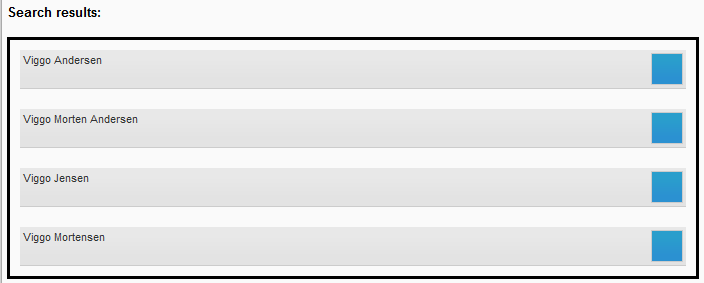
\includegraphics[scale = 0.65]{implementation/figures/results.png}
	\caption{Search results}
	\label{fig:searchresults}
\end{figure}

The search results are listed with the exact match of first and last name first, followed by the closest partial match, which matches both firstname and lastname but with the middle name Morten, and lastly other people called Viggo. The two highest rated matches however both have the weight 2, seeing as they both contain ``Viggo'' and ``Andersen''. There is no exact match checking for names, only for usernames and e-mails, which are not public.

The code for the weighted search is shown below:

\begin{lstlisting}[language=Python,caption=Weighting of the search results]
results = []
# If the search matches a **username** or **email** exactly, add it with high weight, else exclude usernames
try:
	user = User.objects.get(Q(username=request.POST['query'])|Q(email=request.POST['query']))
	profile = user.profile
except (User.DoesNotExist, Profile.DoesNotExist):
	pass
else:
	user_obj = get_user_obj(profile)
	user_obj['weight'] = 100
	results.append(user_obj)

for term in request.POST['query'].split():
	for profile in Profile.objects.filter(
																 Q(firstname__icontains=term)|
																 Q(lastname__icontains=term)):
		added = False
		
		# Duplicate avoidance, and weighting
		for check in results:
			if check['id'] == profile.userLink.id:
				added = True
				check['weight'] = check['weight'] + 1
		if added == False:
			user_obj = get_user_obj(profile)
			user_obj['weight'] = 1
			results.append(user_obj)
					
# Descending weight sort
results.sort(cmp=lambda x,y: cmp(y['weight'], x['weight'])) 
\end{lstlisting}

First, the search checks for exact matches of username and e-mail, gives them a high weigth and adds them to a result array created to contain both exact and partial matches. If there are no exact matches, usernames and e-mails are excluded to ensure that the search can not be abused to find usernames and e-mails of people.
The search is then split up so that each term can be checked with the database seperately. For each term the profiles in the database are then filtered by matches with either firstname or lastname so that partial matches with the search terms can be found. For each profile found the id is checked up to see if this profile occurs in the array already. In case it does, the weight is increased by one. If the match is not in the result array the weight of the match is set to 1, and it is appended to the result array.

Once all matches are weighted the list is sorted by weight using a lambda expression and the resulting list is returned. 